% Options for packages loaded elsewhere
\PassOptionsToPackage{unicode}{hyperref}
\PassOptionsToPackage{hyphens}{url}
%
\documentclass[
]{article}

\usepackage{amsmath,amssymb}
\usepackage{lmodern}
\usepackage{iftex}
\ifPDFTeX
  \usepackage[T1]{fontenc}
  \usepackage[utf8]{inputenc}
  \usepackage{textcomp} % provide euro and other symbols
\else % if luatex or xetex
  \usepackage{unicode-math}
  \defaultfontfeatures{Scale=MatchLowercase}
  \defaultfontfeatures[\rmfamily]{Ligatures=TeX,Scale=1}
\fi
% Use upquote if available, for straight quotes in verbatim environments
\IfFileExists{upquote.sty}{\usepackage{upquote}}{}
\IfFileExists{microtype.sty}{% use microtype if available
  \usepackage[]{microtype}
  \UseMicrotypeSet[protrusion]{basicmath} % disable protrusion for tt fonts
}{}
\makeatletter
\@ifundefined{KOMAClassName}{% if non-KOMA class
  \IfFileExists{parskip.sty}{%
    \usepackage{parskip}
  }{% else
    \setlength{\parindent}{0pt}
    \setlength{\parskip}{6pt plus 2pt minus 1pt}}
}{% if KOMA class
  \KOMAoptions{parskip=half}}
\makeatother
\usepackage{xcolor}
\IfFileExists{xurl.sty}{\usepackage{xurl}}{} % add URL line breaks if available
\IfFileExists{bookmark.sty}{\usepackage{bookmark}}{\usepackage{hyperref}}
\hypersetup{
  pdftitle={arc42 Template},
  hidelinks,
  pdfcreator={LaTeX via pandoc}}
\urlstyle{same} % disable monospaced font for URLs
\usepackage{longtable,booktabs,array}
\usepackage{calc} % for calculating minipage widths
% Correct order of tables after \paragraph or \subparagraph
\usepackage{etoolbox}
\makeatletter
\patchcmd\longtable{\par}{\if@noskipsec\mbox{}\fi\par}{}{}
\makeatother
% Allow footnotes in longtable head/foot
\IfFileExists{footnotehyper.sty}{\usepackage{footnotehyper}}{\usepackage{footnote}}
\makesavenoteenv{longtable}
\usepackage{graphicx}
\graphicspath{ {./images/} }
\makeatletter
\def\maxwidth{\ifdim\Gin@nat@width>\linewidth\linewidth\else\Gin@nat@width\fi}
\def\maxheight{\ifdim\Gin@nat@height>\textheight\textheight\else\Gin@nat@height\fi}
\makeatother
% Scale images if necessary, so that they will not overflow the page
% margins by default, and it is still possible to overwrite the defaults
% using explicit options in \includegraphics[width, height, ...]{}
\setkeys{Gin}{width=\maxwidth,height=\maxheight,keepaspectratio}
% Set default figure placement to htbp
\makeatletter
\def\fps@figure{htbp}
\makeatother
\setlength{\emergencystretch}{3em} % prevent overfull lines
\providecommand{\tightlist}{%
  \setlength{\itemsep}{0pt}\setlength{\parskip}{0pt}}
\setcounter{secnumdepth}{-\maxdimen} % remove section numbering
\ifLuaTeX
  \usepackage{selnolig}  % disable illegal ligatures
\fi

\begin{document}


\includegraphics[width=20mm, height=20mm]{images/arc42-logo.png}
\hypertarget{section-system-scope-and-context}{%
\section{Kontextabgrenzung}\label{section-system-scope-and-context}}

\hypertarget{_fachlicher_kontext}{%
\subsection{Fachlicher Kontext}\label{_fachlicher_kontext}}

\begin {itemize} 
\item Personen können Ausgaben für Gruppen eintragen. Sie setzen dabei für wen und die Applikation berechnet das Saldos für jede der Personen.
\item Eine Person kann in belieb vielen Gruppen, mit beliebig vielen anderen Personen sein. Die UI zeigt eine Gruppenübersicht, mit Liste jeder Gruppe, in der die Person ist und die Detailansicht. Dort werden alle Personen die Mitglied dieser Gruppe sind, mit Saldo wie viel die anderen Personen der Gruppe ihr schuldet, angezeigt.
\item Es kann der Ausgleich einer Gruppe gezeigt werden, s.d. eine Liste von Transaktionen ausgegeben wird, um alle Schulden zu tilgen.
\item Mitglieder können entfernt oder hinzugefügt werden solange die Gruppe offen ist und noch keine Ausgaben getätigt wurden
\item Gruppen können von Mitgliedern jeder Zeit geschlossen werden
\end {itemize}

\hypertarget{_technischer_kontext}{%
\subsection{Technischer Kontext}\label{_technischer_kontext}}

\begin {itemize} 
\item Als Benutzerschnittstelle steht eine Web UI mit Optimierung für PCs, geschützt durch Github OAuth2 zur Verfügung. 
\item Für mobile Geräte ist eine API welche JSON Daten sendet bereitgestelt, um eine optimierte Darstellung durch ein anderes Team zu ermöglichen.
\item Die Persistentz wird durch eine Postgresql Konfiguration mit H2 und Flyway sichergestelt.
\end {itemize}




\hypertarget{section-design-decisions}{%
\section{Architekturentscheidungen}\label{section-design-decisions}}
\begin {itemize} 
\item Wir haben uns für die Personen Klasse entschieden, um die Primitive Obsession zu vermeiden und die berechnungen einfach zu halten. Jedoch stellte sich heraus das diese Entscheidung sich in Hinsicht Persitenz nicht gelohnt hat, wir hielten jedoch daran fest weil das Refactoring am Ende zu viel Aufwand gewesen wäre.
\item Statt der Agregatobjekte benutzen wir Data Transfer Object (DTO) für die Datenbank und den dazu gehörigen Mapper, da unsere Darstellung der Personen als nicht primitives Objekt zu m:n Beziehungen geführt hätte. So wird aus gespeicherten Gruppen und Ausgaben das Agregat zusammen gebaut.
\end {itemize}



\hypertarget{section-design-decisions}{%
\section{Glossar}\label{section-design-decisions}}

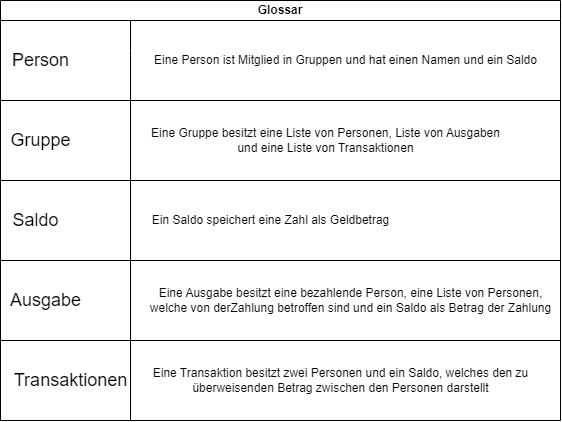
\includegraphics{GlossarFertigFr}

\hypertarget{section-design-decisions}{%
\section{Allgemeine Struktur}\label{section-design-decisions}}

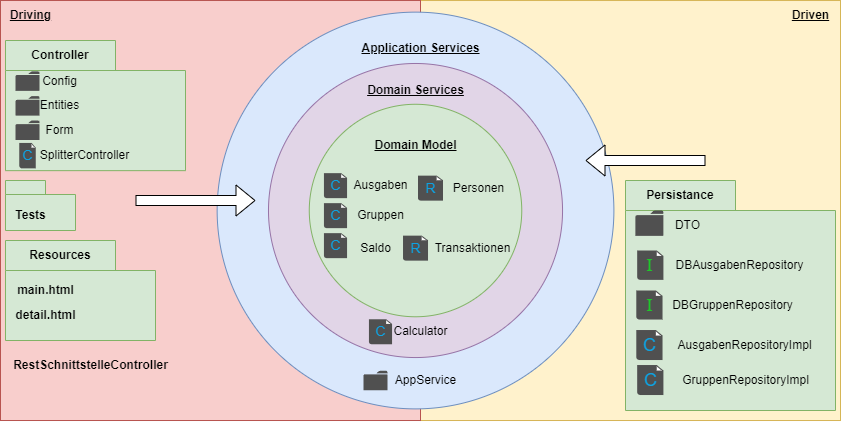
\includegraphics[width=150mm, height=100mm]{StrukturFertig}


\end{document}
